
\section{Characterization of the I-V-Curves}\label{sec:charac}

In order to characterize the assembled sets of \BHSC's, we used the Keithley~2602A~Sourcemeter and ABET~Technologies’ solar simulator SUN~2000. The simulator reproduces the AM 1.5 global reference spectrum and was also equipped with 5 different filters for varying the light intensity. Using the source meter we applied sequences of voltages to the cells and measured the currents resulting from their irradiation. This was done at different levels of intensity of light as well as darkness for which we covered each set with a plastic box.
\subsection{Irradiance calibration}
To ensure that the SUN~2000 was calibrated to yield an irradience of $1\;\text{mW}\!\cdot\text{mm}^{-2}$, we used the Laser~Point PD-500-D9-VIS. With a digital caliper we measured the aperture of the photo diode to have a diameter of $d_p = 9.9(5)\;\text{mm}$. Here we had to assume such a high uncertainty because the construction of the aperture made it very difficult to make out the diameter. This yields an irradiated area of
\begin{equation*}
A_p =  77(8)\;\text{mm}^2.
\end{equation*}
The total power $P_{p0}$ measured by the photo diode at maximum\footnote{This is the intensity corresponding to no filter. We will refer to it with the index 0.} intensity yielded $P_{p0} = 82(1)\;\text{mW}$. So that we arrive at an irradience of
\begin{equation*}
S_{p0} = 1.07(11)\;\frac{\text{mW}}{\text{mm}^2}.
\end{equation*}
Regarding the tools that were at our disposal at this time of the lab, we considered the SUN~2000 to be calibrated correctly. As we will show in section~\ref{sec:discussion} there is external information (see \cite{photodiode}) on the aperture of the photo diode we could not make out at the time of the lab.\mypar
We also conducted this measurement with all filters available to us, in order to see how the modulate the intensity of the light.

\subsection{Crazy stuff}


In order to calculate the open circuit voltage $\Uoc$ and the short circuit current density $\jsc$ for a set of measurements, we did a linear interpolation between the two closest points to the relevant axis \footnote{$j$-axis for $\Uoc$, $U$-axis for $\jsc$}, on each side of it. So if our chosen points for the calculation of $\Uoc$ are $\{(j_1,U_1),(j_2,U_2)\}$ and for $\jsc$ are $\{(j_1^\prime,U_1^\prime),(j_2^\prime,U_2^\prime)\}$, then the formulas for $\Uoc$ and $\jsc$ are as follows.
\begin{align}
\Uoc = \frac{U_2 j_1 - U_1 j_2}{j_1-j_2}\quad \jsc = \frac{U_1^\prime j_2^\prime - U_2^\prime j_1^\prime}{U_1^\prime-U_2^\prime}
\end{align}

To get the maximum power density we simply multiplied the current densities and voltages and took the largest value.
\begin{align}
\Pmax = \max_{i} (j_i\cdot U_i)
\end{align}

The fill factor $FF$ is defined as the ratio of maximum power to the product of open circuit voltage and short circuit current.
\begin{align}
FF = \frac{\Pmax}{\Uoc \cdot \jsc}
\end{align}

In the case of sets $\mathbb{S}_3$ and $\mathbb{S}_\star$ we had multiple working cells. For these we decided to do all calculations with the mean of the current density over the working cells $n$ and include the standard deviation in the uncertainties of our results. The systematic errors of the current $u_{I,\text{sys}}$ and voltage $u_{U,\text{sys}}$ measurements were taken from \cite{keithley}. The uncertainty of the mean of the current density of measurement pair $p$ then is given as:
\begin{align}
u_{\meann{j_p}} = \sqrt{\frac{\sigma_{j,p}^2}{N} + \meann{u_{j_p,\text{sys}}}^2}
\end{align}

With sample size $N$ being the amount of working cells of the set and the systematic error:
\begin{align}
u_{j_{pn},\text{sys}} = \sqrt{ \left( \frac{ u_{I_{pn},\text{sys}}}{A_n}\right)^2+\left( j_{pn}\frac{u_{A_n}}{A_n} \right)^2}
\end{align}

The uncertainty of maximum power and fill factor, as well as short circuit current and open circuit voltage can then be obtained through Gaußian error propagation.

\subsection{First set of \BHSC s}\label{subsec:S1data}

For the first set of \BHSC s $\mathbb{S}_1$, for which only one cell was not shorted, we obtained the following parameters.
\begin{table}[H]\centering
\caption{Key parameters for set $\mathbb{S}_1$ of \BHSC s}
\label{tab:keyparams1}
\begin{tabular}{@{}ccccc@{}}\toprule
$i$ & $\Pmax$ [\textmu W cm$^{-2}$] & $\jsc$ [\textmu A $\mathrm{cm}^{-2}$] & $\Uoc$ [mV] & $FF$ [\%]\\\midrule
0 &  $ 22.1(12) $ & $ -149(5) $ & 424.6(4) & 34.9(21) \\
1 &  $ 15.9(9) $ & $ -124(4) $ & 387.6(3) & 33.0(22) \\
2 &  $ 9.6(5) $ & $ -70.0(24) $ & 343.7(4) & 31.7(23) \\
3 &  $ 2.55(21) $ & $ -37.0(13) $ & 235.2(4) & 29.3(26) \\
4 &  $ 0.75(9) $ & $ -19.7(7) $ & 131.3(3) & 29(4)\\
5 &  $ 0.18(5) $ & $ -10.5(4) $ & 70.93(22) & 24(6) \\\bottomrule
\end{tabular}
\end{table}

%\begin{table}[h]\centering
% \caption{Key parameters for set $\mathbb{S}_1$ of \BHSC s}
% \label{tab:keyparams}
% \begin{tabular}{@{}ccccccc@{}}\toprule
% $i$ & 0 & 1 & 2 & 3 & 4 & 5\\\midrule
% $S_i$ [mW cm$^{-2}$]     & 100 &  & $ -149(5) $ & $  \pm  $ & $  \pm  $ & \\
% $\Pmax$ [$\mu$W cm$^{-2}$] & 22.1(12) & $ 15.9(9) $ & $ 9.6(5) $ & 2.55(21) & 0.75(9) &  0.18(5)\\
% $\jsc$ [$\mu$A cm$^{-2}$]  & - & 9.6(5) & $ -70.0(24) $ & $  \pm  $ & $  \pm  $ & \\
% $\Uoc$ & - & $ 2.55(21) $ & $  $ & $  \pm  $ & $  \pm  $ & \\
% $FF$ & - & $ 0.75(9) $ & $ -19.7(7) $ & $  \pm  $ & $  \pm  $ & \\
% 5 & - & $ 0.18(5) $ & $ -10.5(4) $ & $  \pm  $ & $  \pm  $ & \\\midrule
% \end{tabular}
%\end{table}

In the following figure the current density measurements for four light intensities are shown. The blue rectangle indicates the short circuit current and the open circuit voltage and the orange rectangle the maximum power per area for the measurement at full intensity of incident light.

\begin{figure}[h]\centering
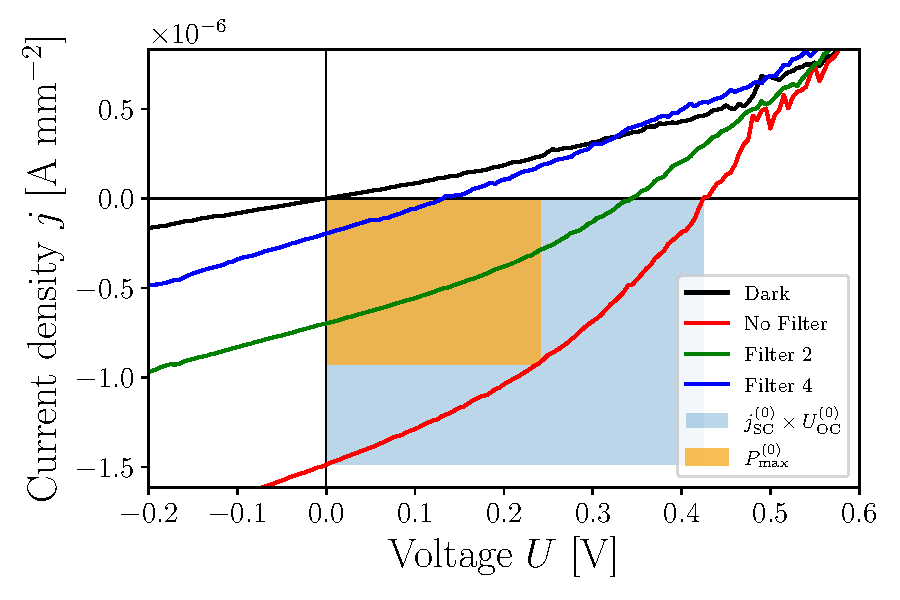
\includegraphics[width=\columnwidth]{../../../IV-Curve-Analysis/OSC1Graph.pdf}
\caption{Current density measurements for the set $\mathbb{S}_1$}
\label{fig:OSC1Graph}
\end{figure}

\subsection{Third set of \BHSC s}

The calculated key parameters for the third set of cells $S_3$ are presented in the same way as in $\ref{subsec:S1data}$.

\begin{table}[h]\centering
\caption{Key parameters for set $\mathbb{S}_3$ of \BHSC s}
\label{tab:keyparams3}
\begin{tabular}{@{}ccccc@{}}\toprule
$i$ & $\Pmax$ [$\mu$W cm$^{-2}$] & $\jsc$ [$\mu$A $\mathrm{cm}^{-2}$] & $\Uoc$ [mV] & $FF$ [\%]\\\midrule
0 &   16.2(14)  &  -111(6)  & 515(5) & 28.2(29) \\
1 &   13.5(13)  &  -95(5)  & 505(5) & 28(3) \\
2 &   7.4(6)  &  -52.7(27)  & 478.9(24) & 29.3(29) \\
3 &   4.0(3)  &  -28.1(14)  & 455.1(29) & 31(3) \\
4 &   2.11(17)  &  -15.0(8)  & 431.2(20) & 33(3)\\
5 &  1.11(9)  &  -8.0(4)  & 406.44(27) & 34(3) \\\bottomrule
\end{tabular}
\end{table}

\begin{figure}[h]\centering
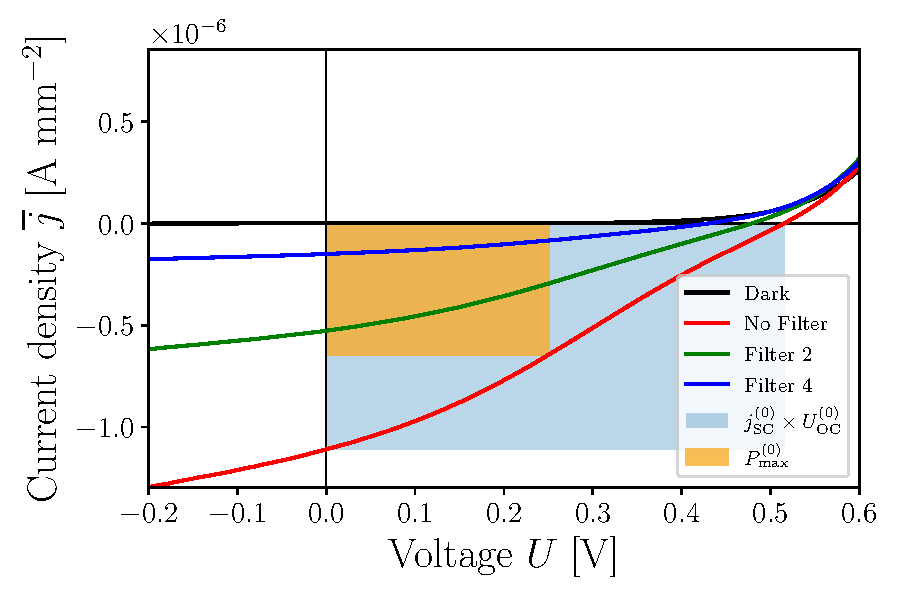
\includegraphics[width=\columnwidth]{../../../IV-Curve-Analysis/OSC2Graph.pdf}
\caption{Current density measurements for the set $\mathbb{S}_3$}
\label{fig:OSC3Graph}
\end{figure}

\subsection{Preassembled set of \BHSC s}

For this set of cells we did not measure the size of the Galinstan droplets, so in order to do the same calculations, we used the average of the measured areas and the average uncertainty as well $A_\star = \langle A_{kn} \rangle_{kn}$, $u_{A_\star} = \langle u_{A_{kn}}  \rangle_{kn}$.

\begin{table}[h]\centering
\caption{Key parameters for set $\mathbb{S}_\star$ of \BHSC s}
\label{tab:keyparamsstar}
\begin{tabular}{@{}ccccc@{}}\toprule
$i$ & $\Pmax$ [$\mu$W cm$^{-2}$] & $\jsc$ [$\mu$A $\mathrm{cm}^{-2}$] & $\Uoc$ [mV] & $FF$ [\%]\\\midrule
0 &   10.4(12)  &  -49(3)  & 747(6) & 28(3) \\
1 &   8.2(8)  &  -41.4(22)  & 716(8) & 27.7(29) \\
2 &   4.7(4)  &  -23.7(12)  & 704(7) & 28.4(29) \\
3 &   2.60(23)  &  -12.8(7)  & 692(8) & 29(3) \\
4 &   1.43(13)  &  -7.0(3)  & 694(7) & 30(3)\\
5 &  0.75(7)  &  -3.73(21)  & 651(10) & 31(4) \\\bottomrule
\end{tabular}
\end{table}

\begin{figure}[H]\centering
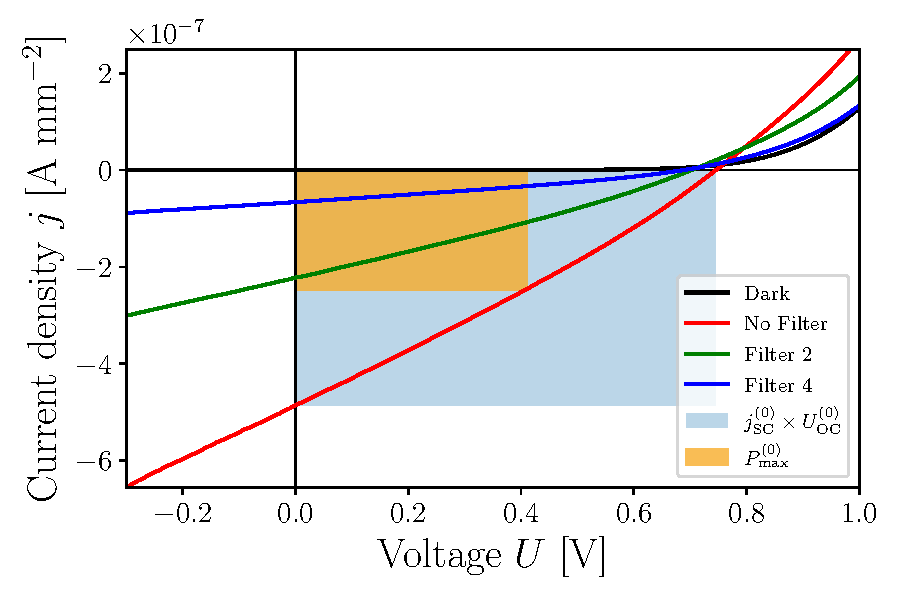
\includegraphics[width=\columnwidth]{../../../IV-Curve-Analysis/OSCPGraph.pdf}
\caption{Current density measurements for the set $\mathbb{S}_\star$}
\label{fig:OSCstarGraph}
\end{figure}

